\chapter{Introducción}

\section{Descripción General}
\par
Este trabajo se fundamenta en dos aspectos: Un aspecto técnico con la implementación de un sistema embebido en chip con microprocesador diseñado
en lenguaje de descripción de hardware y el análisis de esta implementación como base para el desarrollo sistemas de código abierto.
Para implementar el sistema se ha empleado una plataforma basada en sistemas abiertos tanto a nivel de hardware como a nivel del sistema operativo
implantado sobre dicho hardware.
\vspace{0.5cm}
\par
La implementación del sistema se ha llevado a cabo sobre una placa de desarrollo específica, basada en hardware reconfigurable disponible en el
Centro Universitario de Automatización y Robótica (CUDAR) de la Universidad Tecnológica Nacional (UTN) de Córdoba. Aunque la implementación del
sistema de hardware en sí es independiente de la tecnología de implementación.
\vspace{0.5cm}
\par
Inicialmente se analizarán las diferentes alternativas que ofrece el mercado y las comunidades de hardware de código abierto para la
implementación de microprocesadores diseñados en lenguaje de descripción de hardware. Este trabajo ofrece una guía a los diseñadores de
sistemas embebidos para la elección inicial de la arquitectura del sistema, que incluye por lo general como principal componte, al microprocesador.
\vspace{0.5cm}
\par
Luego para llevar a cabo la implementación, se realizó un estudio de componentes que se ajusten a los requerimientos tanto a nivel de hardware como
de sistema operativo.
\vspace{0.5cm}
\par
Con este ejemplo de sistema completo de código abierto se pretende mostrar, tanto que la tecnología de sistemas sobre chip basada en dispositivos
reconfigurables así como los diseños abiertos en hardware y software, son adecuados para la implementación de sistemas reales.

\section{Objetivos}
\subsection{Objetivo General}
\par
Implementar un System on Chip (SoC) Open Source con microprocesador softcore embebido que soporte un sistema operativo libre, con la finalidad de
entregar un sistema integral FPGA-SoC-Sistema Operativo completamente funcional de código abierto, tanto a nivel de hardware como de software.

\subsection{Objetivo Específico}
\begin{itemize}
\item Seleccionar, analizar y determinar la factibilidad de implementación de un microprocesador softcore en FPGA.
\item Seleccionar un SoC Open Source de acuerdo al microprocesador softcore seleccionado.
\item Presentar los Sistemas Operativos Linux y ecOS que poseen las prestaciones funcionales adecuadas para su utilización en Sistemas
Embebidos.
\end{itemize}

\section{Motivación} 
\par
Los sistemas embebidos son aquellos sistemas que implementan una función específica para la cual se tienen que cumplir una serie de restricciones.
Las restricciones principales son el bajo coste y consumo, así como un tamaño y peso lo mas reducído posible.
\vspace{0.5cm}
\par 
Además, muy recientemente, se ha incrementado  significativamente la demanda de sistemas embebidos con diferentes funcionalidades y con mayor
complejidad  en las mismas. Por último, debido a la gran competencia  que hay en este campo, se ha convertido en una restricción fundamental el ser
capaz de reducir significativamente los tiempos de desarrollo de estos sistemas.
\vspace{0.5cm}
\par 
Todos estos problemas han dado lugar a una evolución en la metodología de diseño que se aplica. Así, el principal cambio metodológico ha sido
transformar en aspecto principal del diseño de sistemas embebidos no tanto el diseño del hardware específico sino, más bien, el desarrollo del
software que implementa las diferentes aplicaciones. Esto ha sido posible gracias al avance microelectrónico que hoy en día permite el diseño
completo de un sistema en un chip (System On Chip – SoC) lo que ha permitido partir en el diseño de plataformas hardware base bien desarrolladas.
\vspace{0.5cm}
\par 
Efectivamente, la arquitectura hardware de un sistema embebido en tecnología SoC consiste en uno o varios microprocesadores del sistema sobre los que
se organizan diferentes periféricos necesarios para llevar a cabo la función deseada. Para completar el sistema embebido, la aplicación concreta se
implementa a través del software que se ejecuta en el microprocesador.
\vspace{0.5cm}
\par 
Para lograr las restricciones de reducción de costes y tiempo de desarrollo, las metodologías de diseño de sistemas embebidos parten de una
plataforma hardware base sobre la que se pueden construir un amplio número de aplicaciones. Esta variedad en las aplicaciones se logra gracias a que
las plataformas disponen de múltiples puertos que son capaces de manejar múltiples señales de diferentes tipos. Las plataformas mas comunes hoy en
día siguen siendo los microcontroladores (MCUs) y los procesadores digital de señal (DSPs). Con plataformas hardware basadas en  estos tipos de
componentes, el diseño de la aplicación consiste, primordialmente, en el desarrollo del software.
\vspace{0.5cm}
\par 
Para reducir los tiempos de desarrollo así como para poder emplear esos componentes en funciones de alta complejidad, los fabricantes de los mismos
han hecho un gran esfuerzo en los entornos de desarrollo software. Así, hoy en día, las nuevas series de MCUs se caracterizan porque soportan
sistemas operativos que facilitan significativamente el desarrollo de las varias aplicaciones que va a soportar el sistema final. El mayor
inconveniente que tienen los MCUs es que son plataformas hardware cerradas.
\vspace{0.5cm}
\par 
Como alternativa a las plataformas de hardware cerrado esta la posibilidad de emplear FPGAs. La alta capacidad de integración, el bajo
coste para la fabricación de pequeños lotes y el alto rendimiento, en términos de frecuencia de operación y consumo de potencia, hacen posible
implementar un SoC en este tipo de dispositivo programable. Los SoC que se pueden implementar sobre las FPGAs tienen una serie de ventajas sobre las
plataformas cerradas, como la adaptación a cualquier necesidad específica o la reconfiguración dinámica. Sin embargo, el uso de FPGAs implica
necesariamente un esfuerzo para diseñar la arquitectura hardware que, evidentemente, incrementa el tiempo de desarrollo total del sistema.
\vspace{0.5cm}
\par 
Para hacer realmente útil el diseño de SoC sobre FPGAs en los sistemas embebidos es necesario facilitar la construcción de la arquitectura hardware a
través de buenas metodologías de diseño, así como de un conjunto de herramientas CAD adecuadas. De hecho, hoy en día, el principal esfuerzo que están
haciendo los fabricantes va en la línea de mejorar las herramientas de diseño de SoC sobre FPGAs. Además, existe un alto nivel de competitividad por
encontrar la mejor solución que combine la facilidad de diseño de la arquitectura hardware junto con el mejor rendimiento del sistema final. Ejemplos
de estas herramientas son Xilinx EDK, Altera ESD, etc.. No solo es necesario facilitar el diseño hardware sino también el desarrollo software. Este
es un punto donde, sin duda, hay una gran diferencia de madurez entre los MCUs y el diseño de SoC sobre FPGAs. Como mencionamos anteriormente, los
MCUs soportan sistemas operativos, lo que dota a estas plataformas de una alta versatilidad en cuanto a la funcionalidad y la complejidad que puede
alcanzar un sistema. En contraste, los SoC sobre FPGAs recientemente empiezan a tener soporte para sistemas operativos tales como petalinux
MicroBlaze, o proyectos de portar Linux a Nios o a Lattice Mico32.
\vspace{0.5cm}
\par 
Un alternativa muy interesante de explorar en el diseño de SoC sobre FPGAs es emplear sistemas abiertos tanto  a nivel de hardware como de software.
Los sistemas abiertos se caracterizan porque son tecnológicamente independientes y pueden ser implementables tanto a nivel de FPGAs de bajo coste
como a nivel de ASIC. Existe un grupo de cores Softcore de código abierto que no están limitados por la tecnología. Los cores destacados de
microprocesadores de 32 bits, son los procesadores \textit{SPARC LEON OpenRISC 1200} , y el core de \textit{LatticeMico32}. 
\vspace{0.5cm}
\par 
Usar cores de código abierto va unido a una serie de conceptos como:
\begin {itemize}
	\item \textit{Flexibilidad}  Si el código fuente está disponible, los desarrolladores pueden modificar el código de acuerdo a sus necesidades.
	Además, se produce un flujo constante de ideas que mejoran la calidad del código.
	\item \textit{Fiabilidad y seguridad}  Con muchos programadores a la vez escrutando el mismo trabajo, los errores se detectan y corrigen antes, por lo que
	el producto resultante es mas fiable y eficaz que el comercial.
	\item \textit{Rapidez de desarrollo} Las actualizaciones y ajustes se realizan a través de una comunicación constante vía Internet.
	\item \textit{Relación con el usuario} El programador se acerca mucho más a las necesidades reales de su cliente, y puede crear un producto
	específico para él.
 \end {itemize}

\vspace{0.5cm}
\par  
Todo lo antes mencionado permite obtener un Sistema Integral de código abierto en donde se tiene código HDL, Assembler y C disponible para adaptarse
de acuerdo a los requerimientos del proyecto. 

\section{Importancia del Problema}
\par 
En el diseño de sistemas embebidos se utilizan diferentes procesos dependiendo del tipo de sistema, su arquitectura y el hardware disponible. Una de
las actividades principales en un proceso de diseño de software es la elección del hardware y del sistema operativo, acción que se efectúa antes del
desarrollo del software. Ante tal situación, debe diseñarse el software considerando las restricciones impuestas por las capacidades del hardware.
Los efectos que influyen dichas elecciones comprenden restricciones de temporización sobre el sistema, limitación en la energía disponible,
experiencia del equipo de desarrollo y límites en los costos del sistema final.
\vspace{0.5cm}
\par  
Se está explorando una línea donde se busca dar al diseñador del sistema embebido, una solución flexible en la primera etapa de elección de
la plataforma. Donde a través del análisis de diferentes plataformas de desarrollo Open Source y privativas, se pueda elegir la mejor opción para el
tipo de sistema a desarrollar y los requerimientos de procesamiento. El principal problema que presentan el desarrollo de hardware de código abierto para
no ser adoptado es la dificultad que implican tanto a nivel de diseño hardware como de desarrollo software. 
\vspace{0.5cm}
\par  
Una vez que se ha elegido la plataforma de ejecución para el sistema, se ha diseñado una arquitectura de proceso y se ha determinado una política de
planeamiento, es necesario comprobar que el sistema cumplirá sus con sus requerimientos. El principal problema que presentan el desarrollo de
hardware de código abierto para no ser adoptado es la dificultad que implican tanto a nivel de diseño hardware como de desarrollo software.

\section{Modelo de Desarrollo}
\par
El modelo de desarrollo a utilizar es el Modelo en Espiral (Figura : ~\ref{fig:esquema}) tipificado por Ian Sommerville\cite{Etiqueta00}, fue
originalmente propuesto por Boehm en año 1988, en su artículo " A Spiral Model of Software Development and Enhancement ". Propuso un marco del
proceso de software dirigido por el riesgo.Aquí, el proceso de desarrollo se representa como una espiral, cada ciclo en la espiral representa una
fase del proceso de desarrollo. Por ende, el ciclo más interno puede relacionarse con la factibilidad del sistema, el siguiente ciclo con la
definición de requerimientos, el siguiente ciclo al diseño del sistema, y así sucesivamente. 

\begin{figure}[h!]
 \begin{center}
  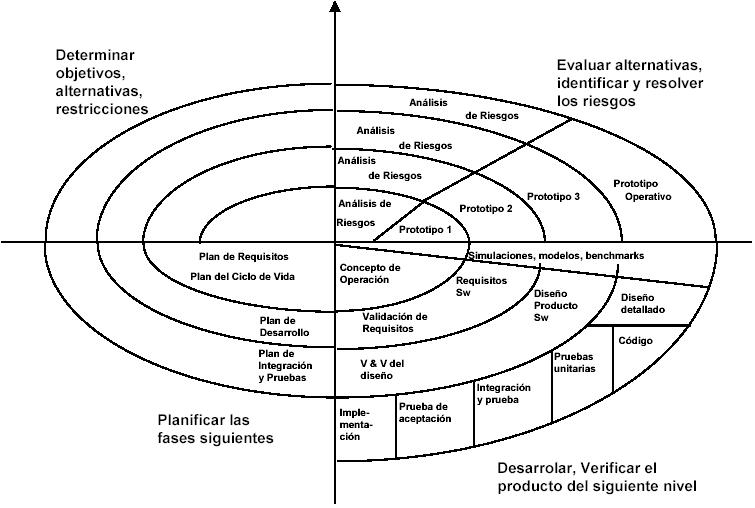
\includegraphics[width=0.5\textwidth,keepaspectratio=true]{./images/ESPIRAL}
  \caption{Etapas del modelo de desarrollo en espiral}
  \label{fig:esquema}
 \end{center}
\end{figure}

\vspace{0.5cm}
\par
Cada ciclo del espiral se divide en 4 sectores:
\begin {itemize}
\item 
\textit{Establecimiento de objetivo} Se definen objetivos específicos para dicha fase del proyecto. Se identifican restricciones en el proceso y el
producto y se traza un plan detallado de gestión. Se identifican los riesgos del proyecto. Dependiendo de estos riesgos, se planean estrategias
alternativas que permitan utilizar otros caminos hacia la solución ante sobre la aparición de problemas asociados a estos riesgos.
\item 
\textit{Validación y reducción del riesgo} En cada uno de los riesgos identificados del proyecto, se realiza un análisis minucioso proponiendo
acciones para reducir dichos riesgos.
\item 
\textit{Desarrollo y validación} Después de una evaluación de riesgos, se elige un modelo de desarrollo para el sistema.
\item 
\textit{Planeamiento}  El proyecto se revisa y se toma una decisión sobre si hay que continuar con otro ciclo de la espiral. Si se opta por continuar,
se trazan los planes para la siguiente fase del proyecto.
\end {itemize}

\vspace{0.5cm}
\par
Como característica principal de esta metodología es que posee una consideración explícita del riesgo. Informalmente, el riesgo significa
sencillamente que algo puede ir mal. Los riegos originan problemas en el proyecto, como los de confección de agendas y excesos en los costos, por lo
tanto, la disminución de riegos es una actividad sumamente importante en la gestión del proyecto. Un ciclo en la espiral comienza con la elaboración
de objetivos, como el rendimiento y la funcionalidad. Entonces se enumeran formas alternativas de alcanzar estos objetivos y las restricciones
impuestas en cada una de ellas. Cada alternativa se evalúa contra cada objetivo y se identifican las fuentes de riegos del proyecto. El siguiente
paso es resolver estos riesgos mediante actividades de recopilación de información como la de detallar más el análisis, la construcción de prototipos
y la simulación. Una vez que se han evaluado los riesgos se llevará a cabo cierto desarrollo, seguido de una actividad de planificación para la
siguiente fase del proceso.

\section{Alcance de Estudio}
\par
Debido al plazo estipulado para el desarrollo del proyecto, el mismo involucra las siguientes etapas: 

\begin {itemize}
	\item Especificación y Análisis de requerimientos.
	\item Análisis de riegos.
	\item Evaluación de Componentes.
	\item Implementación.
	\item Testing.
\end {itemize}

\vspace{0.5cm}
\par
El cumplimiento de cada una de las etapas antes mencionadas, proporcionará un Sistema Integral con hardware y software de código abierto.

\section{Metodología}
\par
Considerando que el objetivo planteado es un desarrollo que se realiza por primera vez en ámbito de la Universidad Nacional de Córdoba, será un
desarrollo experimental y de simulación. La falta de documentación acerca de sistemas de codigo abierto y el hecho ser un desarrollo de vanguardia son
factores que acentúan la decisión de utilización de esta metodología. Sumado a lo dicho anteriormente, en el laboratorio donde se desarrolla este
proyecto no existen antecedentes de trabajos similares que involucren Microprocesadores Softcore.
